\documentclass[14pt,hidelinks]{extarticle}

%%% Поля и разметка страницы %%%
\usepackage{pdflscape}   % Для включения альбомных страниц
\usepackage{geometry} % Для последующего задания полей
\usepackage{setspace} % Для интерлиньяжа
\usepackage[14pt]{extsizes}
\usepackage{titlesec}
\usepackage{tocloft}
\usepackage{enumitem}
\usepackage{fancyhdr}

%%% Кодировки и шрифты %%%
\usepackage{cmap}                    % Улучшенный поиск русских слов в полученном pdf-файле
\usepackage[T2A]{fontenc}	     % Поддержка русских букв
\usepackage[utf8]{inputenc}	     % Кодировка utf8
\usepackage[english=nohyphenation,russian=nohyphenation]{hyphsubst} % Запрет переносов
\usepackage[english, russian]{babel} % Языки: русский, английский
% \usepackage{pscyr}						% Красивые русские шрифты

%%% Математические пакеты %%%
\usepackage{amsthm,amsfonts,amsmath,amssymb,amscd} % Математические дополнения от AMS

%%% Оформление абзацев %%%
\usepackage{indentfirst} % Красная строка

%%% Цвета %%%
\usepackage[usenames]{color}
\usepackage{color}
\usepackage{colortbl}

%%% Таблицы %%%
\usepackage{longtable}		     % Длинные таблицы
\usepackage{multirow,makecell,array} % Улучшенное форматирование таблиц

%%% Общее форматирование
\usepackage{caption}
\captionsetup[figure]{labelsep=space,justification=centering,singlelinecheck=false}
\captionsetup[lstlisting]{labelsep=space,justification=centering,singlelinecheck=false}

\usepackage{soul}                    % Поддержка переносоустойчивых подчёркиваний и зачёркиваний
\usepackage{multicol}

%%% Библиография %%%
\usepackage{cite} % Красивые ссылки на литературу

%%% Гиперссылки %%%
\usepackage[unicode,plainpages=false,pdfpagelabels=false]{hyperref}

%%% Изображения %%%
\usepackage{graphicx} % Подключаем пакет работы с графикой     % Подключаемые пакеты
%%% Макет страницы %%%
\geometry{a4paper,top=20mm,bottom=27mm,left=30mm,right=15mm}
\onehalfspacing
%%% Язык текста %%%
\selectlanguage{russian}

%%% Кодировки и шрифты %%%
\renewcommand{\rmdefault}{ftm} % Включаем Times New Roman

%%% Выравнивание и переносы %%%
\sloppy				% Избавляемся от переполнений
\clubpenalty=10000		% Запрещаем разрыв страницы после первой строки абзаца
\widowpenalty=10000		% Запрещаем разрыв страницы после последней строки абзаца
\interfootnotelinepenalty=10000 % запрет разрыва сносок

%%% Нумерация %%%

\fancyhf{}
\renewcommand{\headrulewidth}{0pt}
\rfoot{\thepage}
\pagestyle{fancy}

%%% Библиография %%%
\makeatletter
\bibliographystyle{utf8gost705u}	% Оформляем библиографию в соответствии с ГОСТ 7.0.5

%%% Изображения %%%
\graphicspath{{images/}} % Пути к изображениям

%%% Содержание %%%
\renewcommand{\cfttoctitlefont}{\hfil\large\bfseries}
\renewcommand\cftsecfont{\normalsize}
\renewcommand\cftsecpagefont{\normalsize}
\renewcommand{\cftsecleader}{\cftdotfill{\cftdotsep}}
\setlength\cftparskip{0pt}
\setlength\cftbeforesecskip{0pt}
\setlength\cftaftertoctitleskip{14pt}

\setlength{\cftsecindent}{0ex}
\setlength{\cftsubsecnumwidth}{5ex}

\setlength{\cftsecnumwidth}{2ex}
\setlength{\cftsubsecnumwidth}{4ex}

%%% Требования ЕСКД/СТП %%%

%%% Размеры заголовков
\titleformat{\section}{\large\bfseries}{\thesection}{1ex}{}
\titleformat{name=\section,numberless}{\large\bfseries\filcenter}{}{1ex}{}
\titlespacing*{\section}{5ex}{14pt}{14pt}

\titleformat{name=\subsection}{\normalsize\bfseries}{\thesubsection}{1ex}{}
\titleformat{name=\subsection,numberless}{\normalsize\bfseries}{}{1ex}{}
\titlespacing*{\subsection}{5ex}{14pt}{14pt}

%%% Размеры текста формул %%%
\DeclareMathSizes{12}{12}{6}{4}

%%% Оформление текста
\setlength{\topskip}{14pt}

\setlength{\parskip}{0pt}
\setlength{\parindent}{5ex}

\setlength{\floatsep}{14pt}
\setlength{\textfloatsep}{14pt}
\setlength{\intextsep}{14pt}
\setlength{\abovecaptionskip}{14pt}
\setlength{\belowcaptionskip}{0pt}

\setlength{\topsep}{0pt}
\setlength{\partopsep}{0pt}
\setlength{\itemsep}{0pt}

\expandafter\def\expandafter\normalsize\expandafter{%
  \normalsize
  \setlength{\abovedisplayskip}{14pt}
  \setlength{\abovedisplayshortskip}{0pt}
  \setlength{\belowdisplayskip}{14pt}
  \setlength{\belowdisplayshortskip}{14pt}
}
% \setlength{}{}                  
\setitemize[0]{leftmargin=7.5ex,itemsep=0pt,topsep=0pt,parsep=0pt}
\renewcommand{\labelitemi}{$-$}

%\numberwithin{equation}{section}
%\renewcommand{\thefigure}{\thesection.\arabic{figure}}
\captionsetup[figure]{labelsep=endash,singlelinecheck=false,skip=0em}
%\renewcommand{\labelenumi}{\thesection.\arabic{enumi}. }

%\renewcommand{\thetable}{\thesection.\arabic{table}} 
\captionsetup[table]{labelsep=endash,justification=raggedright,singlelinecheck=false,skip=0em}
\renewcommand{\arraystretch}{1.1}

%%% Красоты %%%	     % Пользовательские стили

\begin{document}

%%% Переопределение именований %%%
\renewcommand{\abstractname}{Аннотация}
\renewcommand{\alsoname}{см. также}
\renewcommand{\appendixname}{Приложение}
\renewcommand{\bibname}{Литература}
\renewcommand{\ccname}{исх.}
\renewcommand{\chaptername}{Глава}
\renewcommand{\contentsname}{СОДЕРЖАНИЕ}
\renewcommand{\enclname}{вкл.}
\renewcommand{\figurename}{Рисунок}
\renewcommand{\headtoname}{вх.}
\renewcommand{\indexname}{Предметный указатель}
\renewcommand{\listfigurename}{Список рисунков}
\renewcommand{\listtablename}{Список таблиц}
\renewcommand{\pagename}{Стр.}
\renewcommand{\partname}{Часть}
\renewcommand{\seename}{см.}
\renewcommand{\tablename}{Таблица}

\renewcommand{\refname}{СПИСОК ИСПОЛЬЗОВАННЫХ ИСТОЧНИКОВ}	     % Переопределение именований

%%%%%%%%%%%%%%%%%%%%%%%%%%%%%%%%%%%%%%%%%%%%%%%%%%%%%%%%%%%%%%%%

\begin{center}
	\textbf{Типовой расчет} \\ 
	выполнил ст. гр. ****** Петров Ю.А. \\
        Задача №11\\
	Вариант XX 
\end{center}

\section{Условие}

По выборке двумерной случайной величины:

\begin{itemize}
	\item вычислить оценку коэффициента корреляции;
        \item прлверить гипотезу об отсутствии \\
          корреляционной зависимости ($ \alpha = 0.05 $);
	\item вычислить параметры линии регрессии $ \alpha_0 $ и $ \alpha_1 $; 
	\item построить диаграмму рассеивания и линию регрессии;
\end{itemize}

Исходные данные для варианта XX приведены в таблице~\ref{tbl:second_sample}.

\begin{table}[h!]
  \renewcommand{\tabcolsep}{0.6em} 
	\centering
	\caption{Двумерная выборка\label{tbl:second_sample}}
	\begin{tabular}{llllllllll}
          (-0.68; -0.26)	& (-4.03; -2.32)	& (-0.72; 0.47)	& (1.25; 0.82)	& (1.27; -0.81)	\\ 
(-3.57; 0.46)	& (3.00; -2.85)	& (-2.19; 2.71)	& (-4.72; 0.48)	& (4.38; 2.77)	\\ 
(1.16; 2.37)	& (-1.04; 2.03)	& (-0.63; 1.74)	& (-0.07; -0.30)	& (-1.55; 1.85)	\\ 
(1.57; -0.10)	& (-0.27; -0.84)	& (-1.92; -0.17)	& (-0.80; -0.27)	& (-0.30; 3.87)	\\ 
(-2.51; -1.20)	& (0.21; 0.36)	& (2.99; 2.78)	& (2.26; 2.43)	& (1.95; 0.79)	\\ 
(3.27; 0.62)	& (-0.40; 2.71)	& (-0.53; 1.01)	& (0.16; 2.11)	& (3.07; 0.47)	\\ 
(-0.87; -2.17)	& (2.41; -0.85)	& (-0.52; -1.54)	& (0.99; -0.26)	& (0.57; 1.41)	\\ 
(1.47; -0.41)	& (5.76; -1.11)	& (-1.16; 0.95)	& (-1.22; -3.60)	& (3.13; 2.46)	\\ 
(0.90; 0.79)	& (0.77; -3.32)	& (-0.80; -1.46)	& (1.48; -0.69)	& (0.18; 0.25)	\\ 
(2.08; 2.50)	& (-0.99; -2.73)	& (-1.33; 1.70)	& (-2.36; -2.75)	& (-1.82; -2.29)	\\ 
	\\ 

	\end{tabular}
\end{table}

\newpage

\section{Решение}

\subsection{Вычисление точечных оценок параметров двумерной выборки}

Вычислим оценки математических ожиданий по каждой переменной.
\begin{align}
  m^*_X &= \overline{x} = \frac{1}{n} \sum_{i=1}^{n} x_i, &
  m^*_Y &= \overline{y} = \frac{1}{n} \sum_{i=1}^{n} y_i, \\ \nonumber
  m^*_X &= 0.1856, &
  m^*_Y &= 0.2122.
\end{align}

Вычислим оценки дисперсий по каждой переменной.
\begin{equation}
  \begin{aligned}
    D^*_X &= S^2_0(x) = \frac{1}{n-1} \sum_{i=1}^{n} (x_i - \overline{x})^2, \\
    D^*_Y &= S^2_0(y) = \frac{1}{n-1} \sum_{i=1}^{n} (y_i - \overline{y})^2,
  \end{aligned}
\end{equation} 
\begin{equation*}
  \begin{aligned}
    D^*_X &= 4.4893, &
    D^*_Y &= 3.3579.
  \end{aligned}
\end{equation*}

Вычислим оценку корреляционного момента:
\begin{equation}
  K^*_{XY} = \frac{1}{n-1} \sum_{i=1}^{n}{(x_i - \overline{x})(y_i - \overline{y})},
\end{equation} 
\begin{equation*}
  K^*_{XY} = 0.7663.
\end{equation*}

Найдем оценку коэффициента корреляции:
\begin{equation}
  R^*_{XY} = \frac{K^*_{XY}}{\sqrt{S^2_0(x) \cdot S^2_0(y)}},
\end{equation} 
\begin{equation*}
  R^*_{XY} = \dfrac{0.7663}
  {\sqrt{4.4893 \cdot 3.3579}} = 
  0.1974.
\end{equation*}

\subsection{Вычисление интервальной оценки коэффициента корреляции}

Вычислим интервальную оценку коэффициента корреляции с надёжностью $\gamma = 0,95$ по следующей формуле:
\begin{align}
  I_{\gamma} (R_{XY}) &= \left[ \frac{e^{2a}-1}{e^{2a}+1}; \frac{e^{2b}-1}{e^{2b}+1} \right]. 
\end{align}

Для этого в таблице функции Лапласа найдем значение, равное $\frac{\gamma}{2} = 0,475$ и определим значение аргумента, ему соответствующее:
\begin{equation*}
  z_{0,95} = arg \Phi (0,475) = 1,96. 
\end{equation*}

Для вычисления интервальной оценки коэффициента корреляции найдем вспомогательные значения $a, b$ по следующим формулам:
\begin{equation}
  \begin{aligned}
    a &= 0,5 \cdot ln \left( \frac{1+R^*_{XY}}{1-R^*_{XY}} \right) - \frac{z_{\gamma}}{\sqrt{n-3}}, \\
    b &= 0,5 \cdot ln \left( \frac{1+R^*_{XY}}{1-R^*_{XY}} \right) + \frac{z_{\gamma}}{\sqrt{n-3}}, \\
  \end{aligned}
\end{equation}
\begin{equation*}
  \begin{aligned}
    a &= -0.0859, &
    b &= 0.4859.
  \end{aligned}
\end{equation*}

Таким образом, доверительный интервал для коэффициента корреляции имеет вид:
\begin{align}
  I_{\gamma} (R_{XY}) &= \left[ \frac{e^{2a}-1}{e^{2a}+1}; \frac{e^{2b}-1}{e^{2b}+1} \right], \\ \nonumber
  I_{\gamma} (R_{XY}) &= \left[ -0.0857; 
    0.4509 \right]
\end{align}

\newpage 

\subsection{Проверка гипотезы об отсутствии корреляционной зависимости}
Выдвинем двухальтернативную гипотезу об отсутствии корреляционной зависимости 
между величинами $ X $ и $ Y $:

\begin{itemize}
\item $H_0$ --- $ R_{XY} = 0 $: между величинами $ X $ и $ Y $ корреляционная зависимость отсутствует;
\item $H_1$ --- $ R_{XY} = 0 $: между величинами $ X $ и $ Y $ существует корреляционная зависимость.
\end{itemize}

Так как объем выборки велик ($ n \ge 50 $), то вычислим значение критерия по формуле:
\begin{equation}
  Z = \dfrac{|R^*_{XY}| \cdot \sqrt{n}}{1-(R^*_{XY})^2},
\end{equation}
\begin{equation*}
  Z = 1.4236.
\end{equation*}

Определим значение $ Z_\alpha $ из таблицы функции Лапласа ($ \alpha = 0.05 $):
\begin{equation*}
  Z_{0.05} = 1.96.
\end{equation*}

\textbf{Вывод:} так как $ Z = 1.4236 {<}notation{>} Z_{0.05} $,
то гипотеза $H_0$ об отсутствии корреляционной зависимости между величинами $ X $ и $ Y $ принимается (отклоняется).

\newpage

\subsection{Построение линии регрессии}

Уравнение линии регрессии имеет следующий вид:
\begin{equation}
  \overline{y}(x) = a^*_0 + a^*_1 x,
\end{equation} 
где $a^*_1 = \dfrac{K^*_{XY}}{S^2_0(x)},\; a^*_0 = \overline{y} - a^*_1 \cdot \overline{x} $
--- коэффициенты линии регрессии.

\vspace{1em}
Найдем значения $ a^*_1, a^*_0 $:
\begin{equation*}
	\begin{aligned}
		a^*_1 &= 0.1707, &
		a^*_0 &= 0.1805
	\end{aligned}
\end{equation*}

Таким образом, линия регрессии примет вид:
\begin{equation}
  \overline{y}(x) = 0.1805
  + 0.1707 \cdot x
\end{equation}

График линии регрессии изображен на рисунке~\ref{fig:sample_regression}.
\begin{figure}[h!] 
  \centering
  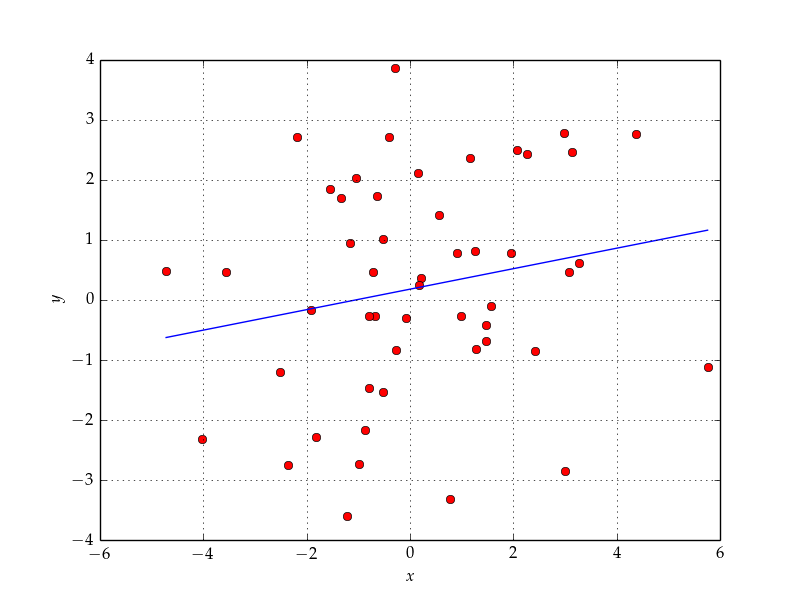
\includegraphics[width=1\linewidth]{pic/sample_regression}
  \caption{График линии регрессии для двумерной случайной величины\label{fig:sample_regression}}
\end{figure}




\end{document}